%%=============================================================================
%% Opstellen projecten
%%=============================================================================

\chapter{Aanmaken blanco project}%
\label{ch:projecten}

Na het opzetten van de ontwikkelomgeving voor zowel native als cross-platform gaan 
we een project opstellen dat we als basis zullen nemen om de functionaliteiten te 
implementeren. In dit hoofdstuk wordt uitgelegd hoe dat gebeurt.

\section{Android Studio}
Bij Android Studio kunnen we in de IDE zelf nieuwe projecten aanmaken om de 
functionaliteiten te maken. Dit doen we met \textit{File > New > New Project...}. 
Hierna krijgen we een overzicht van projecten die we als basis kunnen gebruiken. Ook 
kan er op dit scherm gekozen worden voor welk apparaat de applicatie is.
\begin{figure}[H]
    \centering
    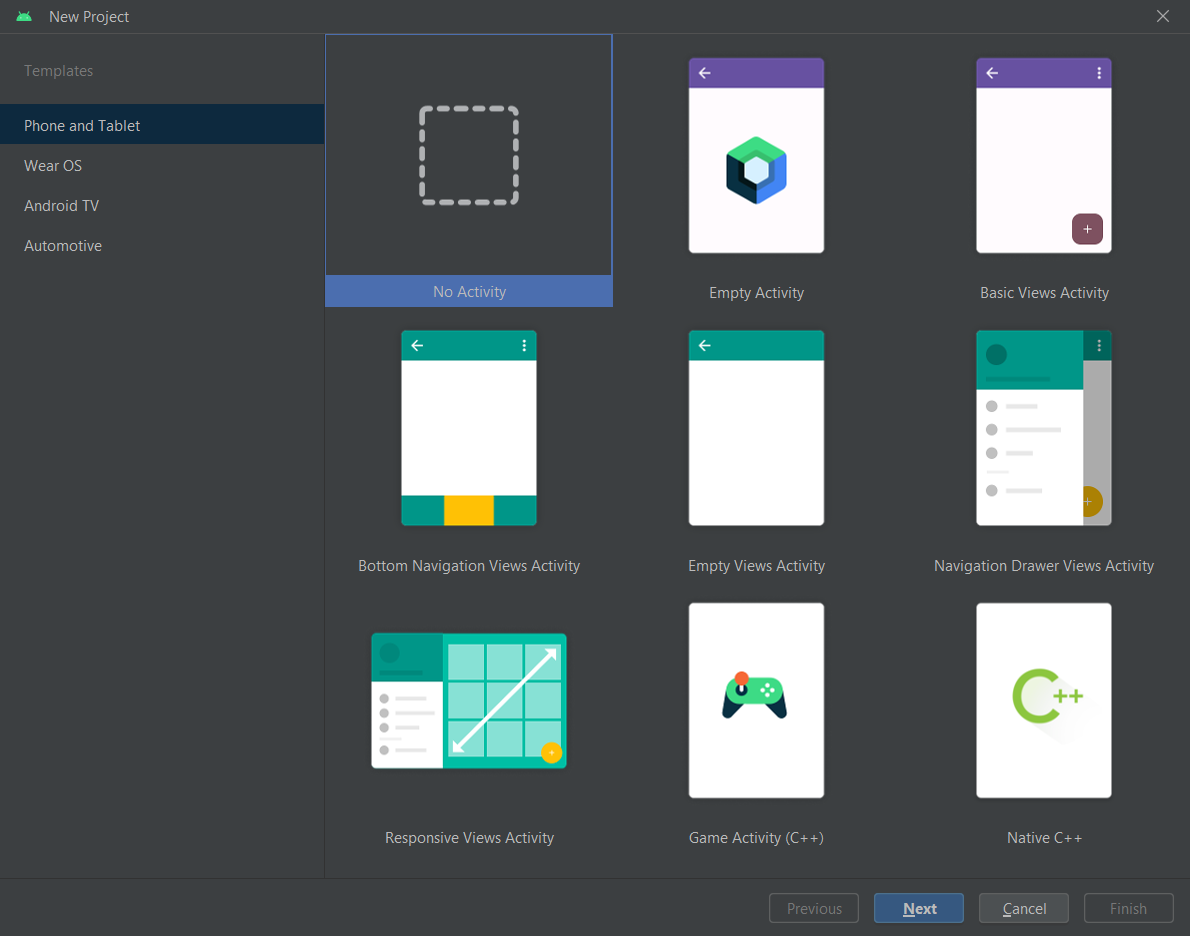
\includegraphics[height=0.35\textheight]{OverzichtProjecten.png}
    \caption{Overzicht startprojecten Android Studio.}
\end{figure}
Afhankelijk van de functionaliteit dat we gaan implementeren zullen we dus andere 
startprojecten kunnen kiezen. Na het kiezen van het startproject geven we een naam, 
programmeertaal en de minimaal ondersteunde Android API. Voor dit onderzoek kiezen we 
voor Kotlin. De naam en minimale ondersteunde Android API speelt hierbij geen rol.

\paragraph{Basisfunctionaliteiten}
\label{par:basisfunctionaliteiten}
Bij de basisfunctionaliteiten zullen we als startproject 
\textbf{Bottom Navigation Views Activity} gebruiken om te kunnen navigeren tussen 
verschillende schermen. Daardoor moeten we zelf geen extra libraries gaan implementeren.

\paragraph{Overige functionaliteiten}
Voor de overige functionaliteiten (camera-integratie, gebruik van sensoren, 
push-notificaties en audio- en videospelers) zullen we als startproject 
\textbf{Empty Activity} gebruiken. Op die manier hebben we de minste \gls{overhead} 
dat de resultaten kan beïnvloeden.

\section{cross-platform project}
Om bij React native een project op te starten gebruiken we volgend commando. 
Deze voeren we uit in de terminal van Visual Studio Code in de gewenste map waar 
het project aangemaakt moet worden.
\begin{minted}{bash}
    npx react-native init <projectnaam>
    // Of
    npx react-native@X.XX.X init <projectnaam> --version X.XX.X
\end{minted}

% komt bovenaan code, andere manier om caption bij code te zetten
% \begin{listing}
%     \begin{minted}{bash}
%         npx react-native init <projectnaam>
%         // Of voor een bepaalde versie Door X.XX.X te veranderen met de gewenste versie
%         npx react-native@X.XX.X init <projectnaam> --version X.XX.X
%     \end{minted}
%     \caption{Nieuw React native project aanmaken.}
%     \label{code:reactnativeprojectopstarten}
% \end{listing}

Dit commando zal een blanco React native project aanmaken waarmee we van start kunnen gaan 
om de functionalieiten te implementeren. Hier kan ook een versie worden meegegeven, 
door \textbf{X.XX.X} in bovenstaande commando te vervangen maken we een project aan 
met de gespecifieerde versie.

